\chapter{CPU, Scheduling, and OS Services}

\section{Measurement overhead}
In this part, we measure the overhead of reading time(read processor cycle counter) and the overhead of using a loop to measure many iterations of an operation. We will use these data to make other experiments more accurate by removing the overhead.

\paragraph{Methodology}
According to the hint, we googled rdtsc instruction and find useful helper functions rdtsc()\cite{rdtsc}, written in inline assembly form that return processor cycle count. 

In order to record the overhead of reading time, we call rdtsc() twice and subtract them. To measure the overhead of using a loop, we apply this method
\lstinputlisting[language=C]{hello.c}
We run it many times, and get the overhead by (end - start) / loops.

\paragraph{Predictions}
As for reading time, I guess the overhead of software is 8 cycles which I get from the inline assembly code. For the hardware layer, I guess it is 9 cycles to perform read, binary operation, write. So total 17 cycles for reading time; 

As for iterations of an operation, I guess software takes 3 cycles to do branch and increment and hardware takes 1 or 2 cycles as overhead, so it is about 5 cycles for iterations.

\paragraph{Results}
We present our measure results.

\begin{center}
\begin{tabular}{l*{6}{c}r}
Operation              & Hardware  & Software  & Overall  & Measured   \\
\hline
Reading time(cycles) & 9 & 8 & 17 & 19  \\
Using a loop (cycles)           & 2 & 3 & 5 & 5 \\
\end{tabular}
\end{center}

\paragraph{Discussion}
My prediction is pretty successful, very close to the measure value. Because we adopted low-overhead mechanism to measure operations and these operations are visible to use, we could follow and predict all the instructions they perform. So our prediction and methodology could get this result. 

\section{Procedure call overhead}
In this part, we measure the overhead of Procedure call. 

\paragraph{Methodology}
In order to get accurate result, we have to tell compiler not to inline the procedure call. So We use this attribute ((noinline)) to tell gcc not to inline procedure call and I turn off OPTIMIZE.

We did not process the arguments in procedure call. We iterate about 100000 times, I record the counter before the loop and record it again after the loop, then remove the iteration overhead.

\paragraph{Predictions}
We predicte when adding more arguments to procedure call, the cycle count should increase linearly. Because we should push each argument to the stack. Besides, procedure call will maintain stack pointers, and instruction like call and ret. When there are no arguments, the cycle should be about 6 cycles, 4 cycles for call, ret and maintain stack pointers and 2 cycles for hardware. When adding one more arguments, we assume hardware and software both add 1 cycles.


\paragraph{Results}
We present our measure results(unit : cycle).

\begin{center}
\begin{tabular}{l*{6}{c}r}
Args              & Hardware  & Software  & Overall  & Measured  & Remove overhead\\
\hline
0 args & 2 & 4 & 6 & 7.1 & 2.1 \\
1 args & 3 & 5 & 8 & 7.3  & 2.3 \\
2 args & 4 & 6 & 10 & 7.7 & 2.7 \\
3 args & 5 & 7 & 12 & 8.6 & 3.6 \\
4 args & 6 & 8 & 14 & 9.3 & 4.3\\
5 args & 7 & 9 & 16 & 10.0 & 5.0\\
6 args & 8 & 10 & 18 & 10.9 & 5.9\\
7 args & 9 & 11 & 20 & 13.1 & 8.1\\
\end{tabular}
\end{center}

\begin{figure}[htbp] %  figure placement: here, top, bottom, or page
   \centering
   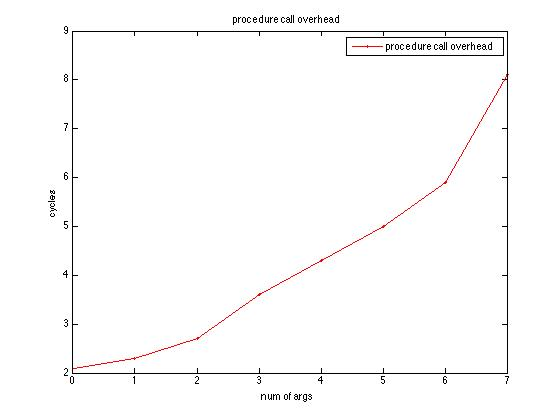
\includegraphics[width=5in]{./pics/pcall.jpg} 
   \caption{procedure call overhead}
   \label{fig:procedure call overhead}
\end{figure}

\paragraph{Discussion}
The measurement statistics is a little strange. Like we have predicted, the overhead for a procedure call scales about linearly with the number of arguments passed in; However, the cycles procedure calls take are less than we have predicted. 

So I tried another methodology. In a loop, first I record the counter, then do procedure call and record again. When calculating, I remove the overhead of counter reading time. But I still get similar results.

I have guessed that compiler may use registers to store parameter in the loop so as to reduce many memory operations. So I look at assembly code but it is pretty regular stack operation.

With the increasing of iteration time, the average cycles decrease a lot. There may be some mechanism like cache in the hardware.

\paragraph{Question} What is the increment overhead of an argument? The increment overhead is about 1 cycle per  argument, pushing parameters to stack.

\section{System call overhead}
In this part, we measure the overhead of System call. There are more than 100 systems in Mac OS and Linux like exit, fork, open and getpid. And the overhead varies a lot. For example, System call like fork will use more cycles than getpid. Because fork will creates a new process by duplicating the calling process which will use much more resources than getpid. So we aim to choose the one that use fewer CPU cycles. The minimal cost can be emulated by measuring the cost of getpid() or getppid().

\paragraph{Methodology}
Because in my operating system getpid() will cache the result, getppid() will not cache the result. So we decided to choose getppid() as our system call overhead measurement target.

The method is similar to measure overhead of procedure call. We iterate about 100000 times, record the counter before the loop and record it again after the loop, then remove the iteration overhead.

\paragraph{Predictions}
As for hardware, it may take 10 cycles to read ppid. As for software, it is hard to estimate. I have implemented system call before. The operations include save current state to memory, trap into kernel, then kernel provide service and finally restore previous state. I measure it as 200 cycles.

\paragraph{Results}
We present our measure results.

\begin{center}
\begin{tabular}{l*{6}{c}r}
Operation              & Hardware  & Software  & Overall  & Measured & Remove Overhead  \\
\hline
getppid() (cycles) & 200 & 10 & 210 & 302 & 297  \\
getpid() (cycles) & ~ & ~ & ~ & 9 & 4  \\
\end{tabular}
\end{center}

\paragraph{Discussion}
Our estimates were lower than the measured result. That is to say, the overhead of user and kernel mode switch is more than we imagine. So, cache some system call results may be a good choice. Because some stupid system call benchmark will repeatedly call getpid ().

\paragraph{Question} How does it compare to the cost of a procedure call? The cost of a system call is much larger than that of a procedure call. Because a system call involves switch between user mode and kernel mode. Furthermore, kernel will provide service to the caller and sometimes will have I/O operations.

\section{Task creation time}
In this part, we measure task creation time, measure the time to create and run both a process and a kernel thread.

\paragraph{Methodology}
For process, we use fork() to create a new process. We iterate 500 times, under Mac OS, if we iterate 1000 times then it will report ERROR so we only iterate 500 times, each iteration we record counter before fork() and after fork() and then get the average time, later remove the iteration overhead.

Things are quiet similar for kernel thread. We use pthread to create a task. Whenever we create a new thread, in the thread function we use pthread\_exit() to kill thread immediately, which will make measurement accurate.

\paragraph{Predictions}
It is difficult to predict accurately. What I am quiet sure is that creating a thread kernel is much more cheaper than creating a process. Because threads share many resources like file descriptors.

For process, I measure the hardware cycles are 200, and the software is 2000.
For thread, I measure the hardware cycles are 50, and the software is 200.

\paragraph{Results}
We present our measure results.

\begin{center}
\begin{tabular}{l*{6}{c}r}
Operation              & Hardware  & Software  & Overall  & Measured   \\
\hline
process & 2000 & 200 & 2200 & 181932  \\
kernel thread    & 200 & 50 & 250 & 16509 \\
\end{tabular}
\end{center}

\paragraph{Discussion}
First, the cost of creating a process is much more expensive than a thread as the data indicated. Because thread is a light process that share many resources so it use fewer CPU cycles.

But I am shocked by the cycles to create a process and thread. I tried gcc -O3 optimisation but did not get any improvement.

\paragraph{Question} How do they compare?
The cost of creating a new process is expensive. Each process has its own address space. Even with COW, there are still many memory copy operation and other overheads. Compared with process, kernel thread can share process resources and can be used in many situations. For example, in a web server, there are many clients and it is impossible to respond to so many clients using process creation model.

